\documentclass[aspectratio=169,11pt,t]{beamer}

% ============================================================
% Theme and typography
% ============================================================

\usetheme{Madrid}
\usecolortheme{default}
\usefonttheme{professionalfonts}

\setbeamertemplate{navigation symbols}{}
\setbeamertemplate{headline}{}

\setbeamertemplate{footline}{%
  \leavevmode\hbox{%
  \begin{beamercolorbox}[wd=.82\paperwidth,ht=2.5ex,dp=1.0ex,leftskip=.8em]{author in head/foot}
    CSCI 6461 --- Computer Systems Architecture
  \end{beamercolorbox}%
  \begin{beamercolorbox}[wd=.18\paperwidth,ht=2.5ex,dp=1.0ex,rightskip=.8em]{date in head/foot}
    \hfill\insertframenumber/\inserttotalframenumber
  \end{beamercolorbox}}
}

\setbeamersize{text margin left=0.65cm,text margin right=0.65cm}

\setbeamerfont{frametitle}{size=\Large, series=\bfseries}
\setbeamerfont{block title}{size=\normalsize, series=\bfseries}
\setbeamertemplate{blocks}[rounded][shadow=false]

\addtobeamertemplate{block begin}{\vspace{0.1em}}{\vspace{0.1em}}
\addtobeamertemplate{block end}{}{\vspace{0.2em}}

\setbeamertemplate{itemize/enumerate body begin}{\setlength{\itemsep}{4pt}}
\setbeamertemplate{itemize/enumerate subbody begin}{\setlength{\itemsep}{2pt}}

% ============================================================
% Packages
% ============================================================

\usepackage[T1]{fontenc}
\usepackage{lmodern}
\IfFileExists{sourcecodepro.sty}{\usepackage[scale=0.92]{sourcecodepro}}{\usepackage{courier}}
\usepackage{amsmath}
\usepackage{booktabs}
\usepackage{array}
\usepackage{colortbl}
\usepackage{tikz}
\usepackage{adjustbox}

\usetikzlibrary{arrows.meta,positioning,shapes.geometric,calc,decorations.pathreplacing}

% ============================================================
% Colors
% ============================================================

\definecolor{navy}{RGB}{24,43,68}
\definecolor{deepblue}{RGB}{45,88,130}
\definecolor{lightblue}{RGB}{235,242,250}
\definecolor{softgray}{RGB}{245,247,250}
\definecolor{darkgray}{RGB}{25,28,32}
\definecolor{gold}{RGB}{200,145,35}
\definecolor{softgreen}{RGB}{226,242,232}
\definecolor{softorange}{RGB}{253,238,215}
\definecolor{softpurple}{RGB}{238,234,250}

\setbeamercolor{palette primary}{bg=navy,fg=white}
\setbeamercolor{palette secondary}{bg=deepblue,fg=white}
\setbeamercolor{frametitle}{bg=navy,fg=white}
\setbeamercolor{title}{fg=white}
\setbeamercolor{subtitle}{fg=white}
\setbeamercolor{author}{fg=white}
\setbeamercolor{date}{fg=white}
\setbeamercolor{titlelike}{fg=white}
\setbeamercolor{block title}{bg=deepblue,fg=white}
\setbeamercolor{block body}{bg=lightblue,fg=darkgray}
\setbeamercolor{normal text}{fg=darkgray,bg=white}

% ============================================================
% Formatting shortcuts
% ============================================================

\setlength{\parskip}{0pt}
\newcommand{\key}[1]{\textbf{#1}}
\newcommand{\bits}[1]{\texttt{#1}}
\newcommand{\hex}[1]{\texttt{0x#1}}
\newcommand{\code}[1]{\texttt{#1}}

\newcommand{\bfld}[5]{%
  \pgfmathsetmacro{\cx}{#1 + #3/2}%
  \fill[#5] (#1,#2) rectangle ++(#3,0.72);%
  \draw[navy,line width=0.7pt] (#1,#2) rectangle ++(#3,0.72);%
  \node[font=\scriptsize,align=center,text=darkgray] at (\cx,#2+0.36) {#4};%
}

\newcommand{\sectiondivider}[2]{%
\begin{frame}[plain]
\begin{tikzpicture}[remember picture,overlay]
\fill[navy] (current page.south west) rectangle (current page.north east);
\fill[gold] (current page.south west) rectangle ([yshift=.15cm]current page.south east);
\end{tikzpicture}
\vspace*{\fill}
\begin{minipage}{0.94\textwidth}
\raggedright
\hyphenpenalty=10000
\exhyphenpenalty=10000
{\color{gold}\large\bfseries #1\par}
\vspace{0.3cm}
{\color{white}\fontsize{22}{26}\selectfont\bfseries #2\par}
\end{minipage}
\vspace*{\fill}
\end{frame}
}

\tikzset{
  unit/.style={draw=navy,line width=0.8pt,rounded corners=2pt,fill=lightblue,minimum width=2.35cm,minimum height=0.82cm,align=center,font=\small},
  state/.style={unit,fill=gold!24},
  logic/.style={unit,fill=softgreen},
  mux/.style={trapezium, trapezium left angle=70, trapezium right angle=110, draw=navy, line width=0.8pt, fill=softorange, minimum width=0.62cm, minimum height=0.95cm, font=\scriptsize, align=center},
  arr/.style={-{Stealth[length=2.2mm]},draw=navy,line width=0.8pt},
  bus/.style={-{Stealth[length=2.2mm]},draw=navy,line width=1.0pt},
  ctrl/.style={-{Stealth[length=2.0mm]},draw=deepblue,line width=0.8pt,dashed}
}
\tikzset{
  memblock/.style={state,minimum width=3.15cm,minimum height=1.05cm},
  regblock/.style={state,minimum width=2.35cm,minimum height=1.45cm}
}


% Reusable register-file symbol based on the ARM datapath convention.
\newcommand{\RegFileSymbol}[1][0.42]{%
\begin{tikzpicture}[
    scale=#1,
    transform shape,
    font=\sffamily\color{black!55},
    thick_line/.style={draw=black!55, ultra thick},
    pin_line/.style={draw=black!55, very thick}
]
    \draw[thick_line] (0,0) rectangle (3.6,4.6);

    \draw[thick_line] (0.3,4.6) -- (0.6,4.3) -- (0.9,4.6);

    \draw[pin_line] (0.6,4.6) -- (0.6,4.9)
      node[above,inner sep=3pt,font=\sffamily\large\color{black!55}] {CLK};

    \draw[pin_line] (1.8,4.6) -- (1.8,4.9);
    \node[below,font=\sffamily\large\color{black!55}] at (1.8,4.6) {WE3};

    \draw[pin_line] (-0.6,3.9) -- (0,3.9);
    \node[right,font=\sffamily\large\color{black!55}] at (0.1,3.9) {A1};

    \draw[pin_line] (-0.6,2.6) -- (0,2.6);
    \node[right,font=\sffamily\large\color{black!55}] at (0.1,2.6) {A2};

    \draw[pin_line] (-0.6,1.6) -- (0,1.6);
    \node[right,font=\sffamily\large\color{black!55}] at (0.1,1.6) {A3};

    \draw[pin_line] (-0.6,0.9) -- (0,0.9);
    \node[right,font=\sffamily\large\color{black!55}] at (0.1,0.9) {WD3};

    \draw[pin_line] (-0.6,0.3) -- (0,0.3);
    \node[right,font=\sffamily\large\color{black!55}] at (0.1,0.3) {PC};

    \draw[pin_line] (3.6,3.9) -- (4.2,3.9);
    \node[left,font=\sffamily\large\color{black!55}] at (3.5,3.9) {RD1};

    \draw[pin_line] (3.6,2.6) -- (4.2,2.6);
    \node[left,font=\sffamily\large\color{black!55}] at (3.5,2.6) {RD2};

    \node[align=center,font=\sffamily\Large\bfseries\color{black!55}]
      at (2.1,1.3) {Register\\[-0.5ex]File};
\end{tikzpicture}%
}


% Reusable instruction-memory symbol.
\newcommand{\InstrMemSymbol}[1][0.42]{%
\begin{tikzpicture}[
    scale=#1,
    transform shape,
    font=\sffamily\color{black!55},
    thick_line/.style={draw=black!55, ultra thick},
    pin_line/.style={draw=black!55, very thick}
]
    % Main Instruction Memory Box
    \draw[thick_line] (0,0) rectangle (3.2,4.2);

    % Left Input
    \draw[pin_line] (-0.6,2.8) -- (0,2.8);
    \node[right,font=\sffamily\large\color{black!55}] at (0.2,2.8) {A};

    % Right Output
    \draw[pin_line] (3.2,2.8) -- (4.0,2.8);
    \node[left,font=\sffamily\large\color{black!55}] at (3.0,2.8) {RD};

    % Vertical Bus Line
    \draw[thick_line] (4.0,0.0) -- (4.0,5.0);

    % External Instr label (vertical)
    \node[align=left,font=\sffamily\large\color{black!55},rotate=-90] at (3.6,3.6) {Instr};

    % Inner Label
    \node[align=center,font=\sffamily\Large\bfseries\color{black!55}] at (1.6,1.4) {Instruction\\[-0.5ex]Memory};
\end{tikzpicture}%
}




% Reusable data-memory symbol.
\newcommand{\DataMemSymbol}[1][0.42]{%
\begin{tikzpicture}[
    scale=#1,
    transform shape,
    font=\sffamily\color{black!55},
    thick_line/.style={draw=black!55, ultra thick},
    pin_line/.style={draw=black!55, very thick}
]
    \draw[thick_line] (0,0) rectangle (3.0,5.0);

    \draw[thick_line] (0.3,5.0) -- (0.6,4.7) -- (0.9,5.0);

    \draw[pin_line] (0.6,5.0) -- (0.6,5.3)
      node[above,font=\sffamily\large\color{black!55}] {CLK};
    \node[below,font=\sffamily\large\color{black!55}] at (1.8,5.0) {WE};

    \draw[pin_line] (-0.6,3.6) -- (0,3.6);
    \node[right,font=\sffamily\large\color{black!55}] at (0.1,3.6) {A};

    \draw[pin_line] (-0.6,0.4) -- (0,0.4);
    \node[right,font=\sffamily\large\color{black!55}] at (0.1,0.4) {WD};

    \draw[pin_line] (3.0,3.6) -- (3.6,3.6);
    \node[left,font=\sffamily\large\color{black!55}] at (2.9,3.6) {RD};

    \node[align=center,font=\sffamily\Large\bfseries\color{black!55}]
      at (1.5,2.2) {Data\\[-0.5ex]Memory};
\end{tikzpicture}%
}



% Reusable ALU symbol.
\newcommand{\ALUSymbol}[1][0.34]{%
\begin{tikzpicture}[
    scale=#1,
    transform shape,
    font=\sffamily\color{black!55},
    thick_line/.style={draw=black!55, ultra thick},
    pin_line/.style={draw=black!55, very thick}
]
    \draw[thick_line]
        (0, 3.0) --
        (2.0, 2.6) --
        (2.0, -0.6) --
        (0, -1.0) --
        (0, 0.6) --
        (1.0, 1.0) --
        (0, 1.4) --
        cycle;

    \draw[pin_line] (-1.8, 2.2) -- (0, 2.2);
    \node[above,font=\sffamily\large\color{black!55},inner sep=2pt] at (-0.9, 2.2) {SrcA};

    \draw[pin_line] (-1.8, -0.2) -- (0, -0.2);
    \node[above,font=\sffamily\large\color{black!55},inner sep=2pt] at (-0.9, -0.2) {SrcB};

    \draw[pin_line] (2.0, 1.0) -- (2.6, 1.0);

    \draw[pin_line] (1.0, 3.5) -- (1.0, 2.8);

    \node[rotate=90,font=\sffamily\Large\color{black!55}] at (1.4, 1.0) {ALU};
\end{tikzpicture}%
}


% Reusable immediate-extension symbol.
\newcommand{\ExtendSymbol}[1][0.42]{%
\begin{tikzpicture}[
    scale=#1,
    transform shape,
    font=\sffamily\color{black!55},
    thick_line/.style={draw=black!55, ultra thick},
    pin_line/.style={draw=black!55, very thick}
]
    \draw[thick_line]
        (0, 0) --
        (4.0, 0) --
        (4.0, 1.2) --
        (0, 0.5) --
        cycle;

    \draw[pin_line] (-0.6, 0.25) -- (0, 0.25);
    \draw[pin_line] (4.0, 0.6) -- (4.6, 0.6);

    \node[align=center,font=\sffamily\Large\bfseries\color{black!55}] at (2.0, 0.45) {Extend};
\end{tikzpicture}%
}

% ============================================================
% Metadata
% ============================================================

\title[Topic 8]{Building a Simple Single-Cycle RISC Datapath}
\subtitle{State elements, datapath components, control signals, and AArch64 instruction flow}
\author{Computer Systems Architecture}
\date{}

% ============================================================
% Document
% ============================================================

\begin{document}

% ============================================================
% Slide 1
% ============================================================

\begin{frame}[plain]
\begin{tikzpicture}[remember picture,overlay]
\fill[navy] (current page.south west) rectangle (current page.north east);
\fill[gold] (current page.south west) rectangle ([yshift=.15cm]current page.south east);
\end{tikzpicture}
\vspace*{\fill}
\begin{minipage}{0.88\textwidth}
{\color{gold}\normalsize\bfseries CSCI 6461 \;|\; Computer Systems Architecture \;|\; TOPIC 8\par}
\vspace{0.25cm}
{\color{white}\fontsize{24}{28}\selectfont\bfseries Building a Simple Single-Cycle\\[0.08cm]RISC Datapath\par}
\vspace{0.35cm}
{\color{white!80}\large AArch64-style datapath construction using one-cycle execution\\and a worked \code{ldr} instruction path\par}
\end{minipage}
\vfill
{\color{white!70}\small Dr. J. Burns\par}
\vspace*{\fill}
\end{frame}

% ============================================================
% Slide 2
% ============================================================

\begin{frame}{Topic 8 Outline}
\setbeamertemplate{enumerate item}{\arabic{enumi}.}
\begin{enumerate}\setlength{\itemsep}{8pt}
  \item \key{Single-Cycle Microarchitecture}
  \begin{itemize}
    \item Architectural state, combinational logic, and one-cycle execution.
  \end{itemize}
  \item \key{Datapath State Elements}
  \begin{itemize}
    \item PC, instruction memory, register file, ALU, immediate generation, data memory.
  \end{itemize}
  \item \key{Worked Load Path}
  \begin{itemize}
    \item Step-by-step execution of \code{ldr x7, [x5, \#8]}.
  \end{itemize}
  \item \key{Extending the Datapath}
  \begin{itemize}
    \item Store, data-processing, branch paths, and the control signals that select them.
  \end{itemize}
\end{enumerate}
\end{frame}

% ============================================================
% Slide 3
% ============================================================

\sectiondivider{PART 1}{Single-Cycle Microarchitecture}

% ============================================================
% Slide 4
% ============================================================

\begin{frame}{Microarchitecture}
\large
\begin{itemize}\setlength{\itemsep}{7pt}
  \item The \key{ISA} defines the instructions visible to software.
  \item The \key{microarchitecture} is the hardware organization that executes those instructions.
  \item A single-cycle datapath is one microarchitectural implementation of the AArch64 ISA.
  \item The datapath moves values through memories, registers, ALUs, and multiplexers.
  \item The control unit interprets the instruction and selects the datapath actions.
  \item Later implementations can use pipelining while preserving the same ISA behavior.
\end{itemize}
\end{frame}

% ============================================================
% Slide 5
% ============================================================

\begin{frame}{Architectural State as a Finite-State Machine}
\vspace{-0.05cm}
\begin{center}
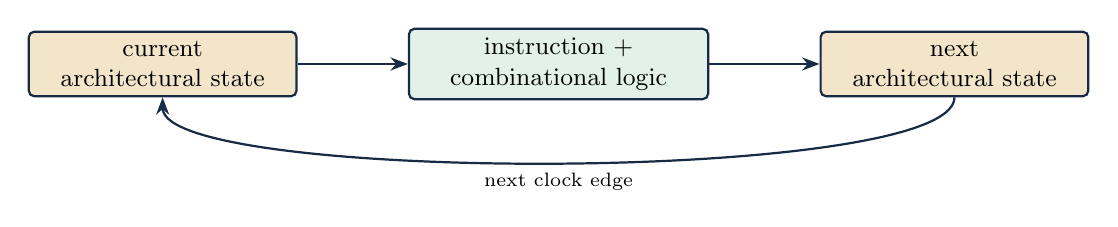
\begin{tikzpicture}[node distance=1.4cm,font=\small]
  \node[state,minimum width=3.4cm] (s0) {current\\architectural state};
  \node[logic,right=of s0,minimum width=3.8cm] (comb) {instruction +\\combinational logic};
  \node[state,right=of comb,minimum width=3.4cm] (s1) {next\\architectural state};
  \draw[bus] (s0) -- (comb);
  \draw[bus] (comb) -- (s1);
  \draw[arr] (s1.south) .. controls +(0,-1.1) and +(0,-1.1) .. node[below,font=\scriptsize]{next clock edge} (s0.south);
\end{tikzpicture}
\end{center}
\vspace{0.1cm}
\begin{itemize}\setlength{\itemsep}{6pt}
  \item State elements hold the visible machine state between cycles.
  \item Combinational logic computes the next state from the current state and instruction.
  \item A clock edge commits the new state.
\end{itemize}
\end{frame}

% ============================================================
% Slide 6
% ============================================================

\begin{frame}{Single-Cycle Execution}
\large
\begin{itemize}\setlength{\itemsep}{7pt}
  \item One instruction completes in one clock cycle.
  \item Fetch, decode, execute, memory access, and writeback all fit in that cycle.
  \item State is updated at the clock edge at the end of the cycle.
  \item The clock period must be long enough for the slowest supported instruction.
\end{itemize}
\vspace{0.2cm}
\begin{center}
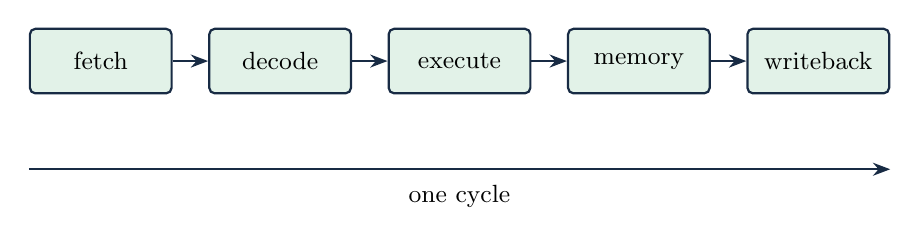
\begin{tikzpicture}[font=\small,node distance=0.45cm]
  \node[logic,minimum width=1.8cm] (f) {fetch};
  \node[logic,right=of f,minimum width=1.8cm] (d) {decode};
  \node[logic,right=of d,minimum width=1.8cm] (e) {execute};
  \node[logic,right=of e,minimum width=1.8cm] (m) {memory};
  \node[logic,right=of m,minimum width=1.8cm] (w) {writeback};
  \draw[arr] (f)--(d);
  \draw[arr] (d)--(e);
  \draw[arr] (e)--(m);
  \draw[arr] (m)--(w);
  \draw[arr] ([yshift=-0.95cm]f.south west) -- ([yshift=-0.95cm]w.south east)
    node[midway,below=2pt]{one cycle};
\end{tikzpicture}
\end{center}
\end{frame}

% ============================================================
% Slide 7
% ============================================================

\begin{frame}{AArch64 State Used Here}
\begin{columns}[T,onlytextwidth]
\column{0.48\textwidth}
\begin{itemize}\setlength{\itemsep}{6pt}
  \item \key{PC}: address of the current instruction.
  \item \key{Register file}: 32 architectural register numbers, 5 bits each.
  \item \key{NZCV}: condition flags used by conditional branches.
\end{itemize}
\column{0.48\textwidth}
\begin{itemize}\setlength{\itemsep}{6pt}
  \item The PC is modeled as a separate register, not as \code{x15} or \code{r15}.
  \item \code{x31} is interpreted as \code{sp} or \code{xzr}, depending on the instruction form.
  \item This simplified datapath treats the register file as two read ports and one write port.
\end{itemize}
\end{columns}
\vspace{0.15cm}
AArch64 differs from the older ARM32 teaching model: there is no general-purpose \code{r15} program counter register.
\end{frame}

% ============================================================
% Slide 8
% ============================================================

\begin{frame}{Instruction Subset}
\large
\begin{itemize}\setlength{\itemsep}{7pt}
  \item \key{Memory}: \code{ldr xT, [xN, \#imm]} and \code{str xT, [xN, \#imm]} using unsigned scaled offsets.
  \item \key{Data processing}: \code{add}, \code{sub}, \code{and}, \code{orr} in register and simple immediate forms.
  \item \key{Control flow}: \code{b label} and simple conditional branches such as \code{b.eq label}.
  \item The load instruction is traced first because it exercises fetch, register read, immediate generation, ALU address calculation, data memory, and writeback.
\end{itemize}
\vspace{0.15cm}
This is not a full AArch64 implementation. It is a small datapath that is large enough to show the hardware pattern.
\end{frame}

% ============================================================
% Slide 9
% ============================================================

\sectiondivider{PART 2}{State Elements and Core Datapath Blocks}

% ============================================================
% Slide 10
% ============================================================

\begin{frame}{Datapath and Control}
\vspace{-0.05cm}
\begin{center}
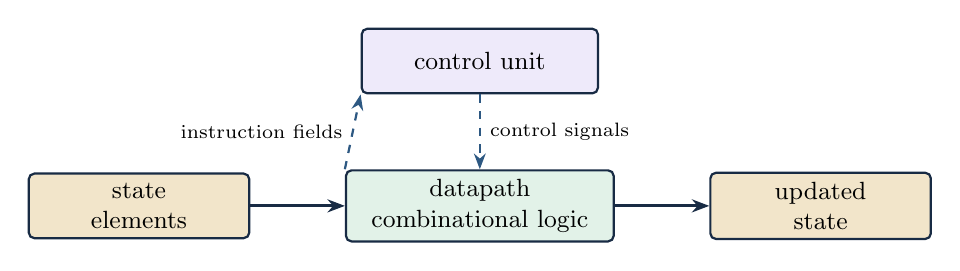
\begin{tikzpicture}[node distance=1.2cm,font=\small]
  \node[state,minimum width=2.8cm] (state) {state\\elements};
  \node[logic,right=of state,minimum width=3.4cm] (dp) {datapath\\combinational logic};
  \node[logic,above=0.95cm of dp,minimum width=3.0cm,fill=softpurple] (ctrl) {control unit};
  \node[state,right=of dp,minimum width=2.8cm] (new) {updated\\state};
  \draw[bus] (state)--(dp); \draw[bus] (dp)--(new);
  \draw[ctrl] (ctrl)--node[right,font=\scriptsize]{control signals}(dp);
  \draw[ctrl] (dp.north west)--node[left,font=\scriptsize]{instruction fields}(ctrl.south west);
\end{tikzpicture}
\end{center}
\vspace{0.1cm}
\begin{itemize}\setlength{\itemsep}{6pt}
  \item The datapath contains the values and arithmetic.
  \item The control unit chooses which path the current instruction uses.
\end{itemize}
\end{frame}

% ============================================================
% Slide 11
% ============================================================

\begin{frame}{Register File}
\begin{columns}[T,onlytextwidth]
\column{0.45\textwidth}
\begin{itemize}\setlength{\itemsep}{6pt}
  \item \code{A1} and \code{A2} select the two registers to read.
  \item \code{A3} selects the register to write.
  \item \code{WD3} carries the write data.
  \item \code{WE3} enables the write at the clock edge.
  \item \code{RD1} and \code{RD2} carry the two read values.
\end{itemize}

\column{0.52\textwidth}
\begin{center}
\RegFileSymbol[0.48]
\end{center}
\end{columns}
\end{frame}

% ============================================================
% Slide 12
% ============================================================

\begin{frame}{State Elements}
\begin{center}
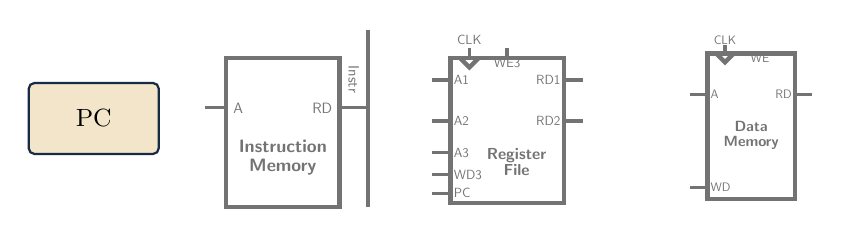
\begin{tikzpicture}[font=\small]
  \node[state,minimum width=1.65cm,minimum height=0.9cm] (pc) at (0,0) {PC};
  \node[draw=none,inner sep=0pt] (imem) at (2.45,0) {\InstrMemSymbol[0.45]};
  \node[draw=none,inner sep=0pt] (rf) at (5.25,0) {\RegFileSymbol[0.40]};
  \node[draw=none,inner sep=0pt] (dmem) at (8.35,0) {\DataMemSymbol[0.37]};
\end{tikzpicture}
\end{center}
\vspace{0.2cm}
\begin{itemize}\setlength{\itemsep}{6pt}
  \item The PC supplies the address for instruction fetch.
  \item The register file stores integer register values.
  \item Data memory is read by \code{ldr} and written by \code{str}.
  \item Writes to architectural state happen at the end of the cycle.
\end{itemize}
\end{frame}

% ============================================================
% Slide 13
% ============================================================

\begin{frame}{Program Counter and Instruction Memory}
\begin{center}
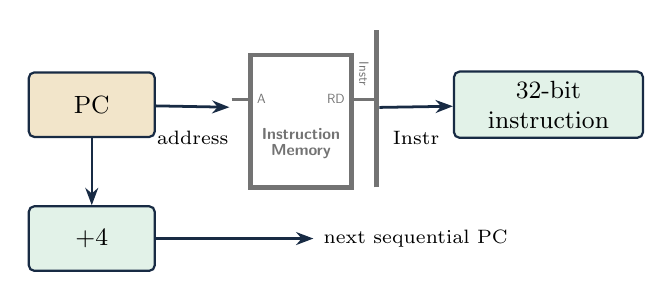
\begin{tikzpicture}[font=\small]
  \node[state,minimum width=1.6cm] (pc) at (0,0.6) {PC};
  \node[draw=none,inner sep=0pt] (imem) at (2.7,0.55) {\InstrMemSymbol[0.40]};
  \node[logic,minimum width=2.4cm] (instr) at (5.8,0.6) {32-bit\\instruction};
  \node[logic,minimum width=1.6cm] (add4) at (0,-1.1) {+4};
  \draw[bus] (pc)--node[below=5pt,font=\scriptsize]{address}(imem);
  \draw[bus] (imem)--node[below=5pt,font=\scriptsize]{Instr}(instr);
  \draw[arr] (pc)--(add4);
  \draw[arr] (add4.east) -- ++(2.0,0) node[right,font=\scriptsize]{next sequential PC};
\end{tikzpicture}
\end{center}
\vspace{0.1cm}
AArch64 instructions are 4 bytes, so the sequential PC value is \(PC+4\).
\end{frame}

% ============================================================
% Slide 14
% ============================================================

\begin{frame}{ALU and Immediate Generator}
\begin{columns}[T,onlytextwidth]
\column{0.48\textwidth}
\begin{block}{ALU}
\begin{itemize}\setlength{\itemsep}{4pt}
  \item computes add/subtract/logical results;
  \item produces address calculations for loads and stores;
  \item can produce NZCV flags for flag-setting forms.
\end{itemize}
\end{block}
\column{0.48\textwidth}
\begin{block}{Immediate Generator}
\begin{itemize}\setlength{\itemsep}{4pt}
  \item extracts immediate fields from the instruction;
  \item scales load/store offsets when required;
  \item sign-extends branch offsets.
\end{itemize}
\end{block}
\end{columns}
\vspace{0.15cm}
\begin{center}
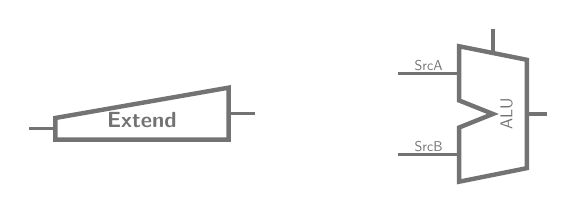
\begin{tikzpicture}[font=\small]
  \node[draw=none,inner sep=0pt] (imm) at (0,0) {\ExtendSymbol[0.55]};
  \node[draw=none,inner sep=0pt] (alu) at (4.2,0.1) {\ALUSymbol[0.43]};
\end{tikzpicture}
\end{center}
\end{frame}

% ============================================================
% Slide 15
% ============================================================

\begin{frame}{AArch64 Immediate Modes in This Datapath}
\small
\begin{center}
\rowcolors{2}{blue!6}{white}
\begin{tabular}{lll}
\toprule
Instruction form & Immediate field & Datapath value \\
\midrule
\code{ldr/str xT, [xN, \#imm]} & \code{imm12} & zero-extended and scaled by access size \\
\code{add/sub xD, xN, \#imm} & \code{imm12} & zero-extended immediate \\
\code{b label} & \code{imm26} & sign-extended, shifted left by 2 \\
\code{b.cond label} & \code{imm19} & sign-extended, shifted left by 2 \\
\bottomrule
\end{tabular}
\end{center}
\vspace{0.15cm}
The control unit selects the immediate mode using an \code{ImmSrc} signal.
\end{frame}

% ============================================================
% Slide 16
% ============================================================

\begin{frame}{Data Memory}
\large
\begin{itemize}\setlength{\itemsep}{7pt}
  \item The ALU computes the effective address from a base register and offset.
  \item \code{ldr} reads data memory and writes the loaded value to the register file.
  \item \code{str} reads a register value and writes that value to data memory.
  \item The simplified model treats memory as a separate instruction memory and data memory.
  \item The same address-generation path is used by both \code{ldr} and \code{str}.
\end{itemize}
\end{frame}

% ============================================================
% Slide 17
% ============================================================

\sectiondivider{PART 3}{Worked Load Path}

% ============================================================
% Slide 18
% ============================================================

\begin{frame}{Load Example}
\large
\code{ldr x7, [x5, \#8]}

\vspace{0.22cm}
\begin{itemize}\setlength{\itemsep}{7pt}
  \item Read the base address from \code{x5}.
  \item Add the byte offset \code{8} to form the effective address.
  \item Read 8 bytes from data memory.
  \item Write the loaded 64-bit value into \code{x7}.
  \item Update the PC to the next sequential instruction at the end of the cycle.
\end{itemize}
\vspace{0.12cm}
For a 64-bit AArch64 load with unsigned offset, the encoded \code{imm12} is \(8/8 = 1\).
\end{frame}

% ============================================================
% Slide 19
% ============================================================

\begin{frame}{Load Instruction Fields}
\small
\code{ldr x7, [x5, \#8]} is encoded as \hex{F94004A7}.

\vspace{0.18cm}
\begin{center}
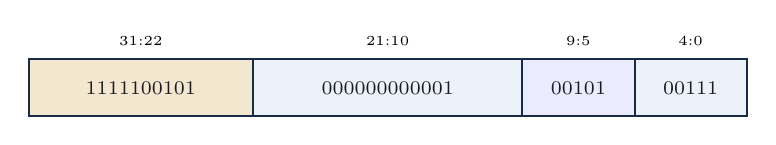
\begin{tikzpicture}[x=0.285cm,y=1cm]
  \bfld{0}{0}{10}{1111100101}{gold!22}
  \bfld{10}{0}{12}{000000000001}{lightblue}
  \bfld{22}{0}{5}{00101}{blue!8}
  \bfld{27}{0}{5}{00111}{lightblue}
  \node[font=\tiny] at (5,0.95) {31:22};
  \node[font=\tiny] at (16,0.95) {21:10};
  \node[font=\tiny] at (24.5,0.95) {9:5};
  \node[font=\tiny] at (29.5,0.95) {4:0};
\end{tikzpicture}
\end{center}
\vspace{0.1cm}
\begin{center}
\rowcolors{2}{blue!6}{white}
\begin{tabular}{lll}
\toprule
Field & Value & Meaning \\
\midrule
opcode/form & \bits{1111100101} & 64-bit load, unsigned immediate \\
\code{imm12} & \bits{000000000001} & scaled offset 1, meaning 8 bytes \\
\code{Rn} & \bits{00101} & base register \code{x5} \\
\code{Rt} & \bits{00111} & destination register \code{x7} \\
\bottomrule
\end{tabular}
\end{center}
\end{frame}

% ============================================================
% Slide 20
% ============================================================

\begin{frame}{Step 1: Fetch the Instruction}
\begin{center}
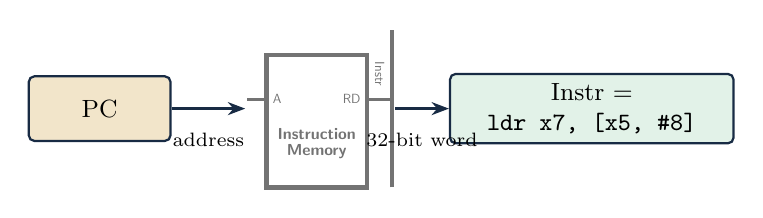
\begin{tikzpicture}[font=\small]
  \node[state,minimum width=1.8cm] (pc) at (0,0) {PC};
  \node[draw=none,inner sep=0pt] (imem) at (2.8,0) {\InstrMemSymbol[0.40]};
  \node[logic,minimum width=3.6cm] (instr) at (6.25,0) {Instr =\\\code{ldr x7, [x5, \#8]}};

  \draw[bus] (pc) -- node[below=5pt,font=\scriptsize]{address} (imem);
  \draw[bus] (imem) -- node[below=5pt,font=\scriptsize]{32-bit word} (instr);
\end{tikzpicture}
\end{center}
\vspace{0.25cm}
The PC supplies the instruction address. Instruction memory returns the 32-bit AArch64 instruction word.
\end{frame}

% ============================================================
% Slide 21
% ============================================================

\begin{frame}{Step 2: Decode Register Fields}
\begin{center}
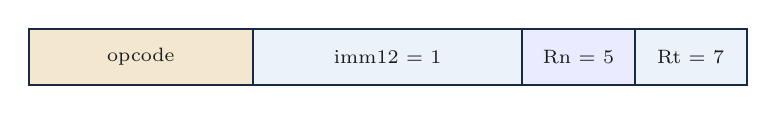
\begin{tikzpicture}[x=0.285cm,y=1cm]
  \bfld{0}{0}{10}{opcode}{gold!22}
  \bfld{10}{0}{12}{imm12 = 1}{lightblue}
  \bfld{22}{0}{5}{Rn = 5}{blue!8}
  \bfld{27}{0}{5}{Rt = 7}{lightblue}
\end{tikzpicture}
\end{center}
\vspace{0.15cm}
\begin{itemize}\setlength{\itemsep}{6pt}
  \item \code{Rn} selects the base register: \code{x5}.
  \item \code{Rt} selects the destination register: \code{x7}.
  \item The register file reads \code{x5} while the rest of the datapath computes the offset and address.
\end{itemize}
\end{frame}

% ============================================================
% Slide 22
% ============================================================

\begin{frame}{Step 3: Read the Base Register}
\begin{center}
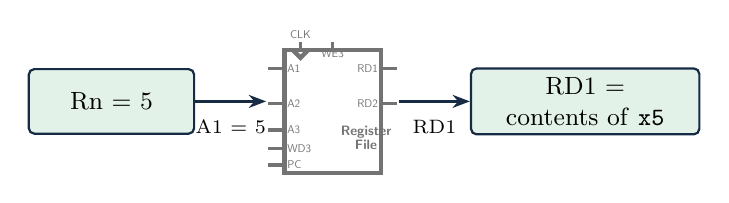
\begin{tikzpicture}[node distance=0.9cm,font=\small]
  \node[logic,minimum width=2.1cm] (field) {Rn = 5};
  \node[draw=none,inner sep=0pt,right=of field] (rf) {\RegFileSymbol[0.34]};
  \node[logic,right=0.9cm of rf,minimum width=2.9cm] (rd1) {RD1 =\\contents of \code{x5}};
  \draw[bus] (field.east)--node[below=3pt,font=\scriptsize]{A1 = 5}(rf.west);
  \draw[bus] (rf.east)--node[below=3pt,font=\scriptsize]{RD1}(rd1.west);
\end{tikzpicture}
\end{center}
\vspace{0.2cm}
The base address is not embedded in the instruction. The instruction names the register that holds the base address.
\end{frame}

% ============================================================
% Slide 23
% ============================================================

\begin{frame}{Step 4: Generate the Offset}
\begin{columns}[T,onlytextwidth]
\column{0.47\textwidth}
\begin{itemize}\setlength{\itemsep}{6pt}
  \item Field value: \code{imm12 = 1}.
  \item Access size: 8 bytes, because this is \code{ldr x}.
  \item Byte offset: \(1 \times 8 = 8\).
\end{itemize}
\column{0.50\textwidth}
\begin{center}
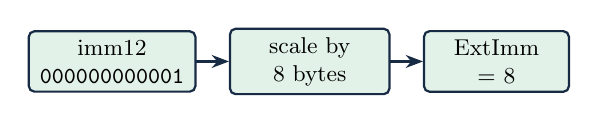
\begin{tikzpicture}[node distance=0.45cm,font=\small,scale=0.92,transform shape]
  \node[logic,minimum width=2.3cm] (imm) {imm12\\\bits{000000000001}};
  \node[logic,right=of imm,minimum width=2.2cm] (scale) {scale by\\8 bytes};
  \node[logic,right=of scale,minimum width=2.0cm] (out) {ExtImm\\= 8};
  \draw[arr] (imm)--(scale); \draw[arr] (scale)--(out);
\end{tikzpicture}
\end{center}
\end{columns}
\vspace{0.15cm}
AArch64 unsigned load/store offsets are scaled by the access size.
\end{frame}

% ============================================================
% Slide 24
% ============================================================

\begin{frame}{Step 5: Compute the Effective Address}
\begin{center}
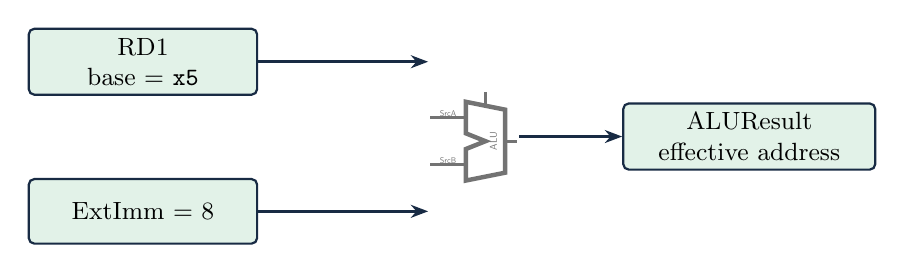
\begin{tikzpicture}[font=\small]
  \node[logic,minimum width=2.9cm] (base) at (0,0.9) {RD1\\base = \code{x5}};
  \node[logic,minimum width=2.9cm] (imm) at (0,-1.0) {ExtImm = 8};
  \node[draw=none,inner sep=0pt] (alu) at (4.2,-0.05) {\ALUSymbol[0.25]};
  \node[logic,minimum width=3.2cm] (addr) at (7.7,-0.05) {ALUResult\\effective address};
  \draw[bus] (base.east)--(alu.west |- base.east);
  \draw[bus] (imm.east)--(alu.west |- imm.east);
  \draw[bus] (alu.east)--(addr.west);
\end{tikzpicture}
\end{center}
\vspace{0.2cm}
For a load or store, the ALU is used as an address adder.
\end{frame}

% ============================================================
% Slide 25
% ============================================================

\begin{frame}{Step 6: Read Data Memory}
\begin{center}
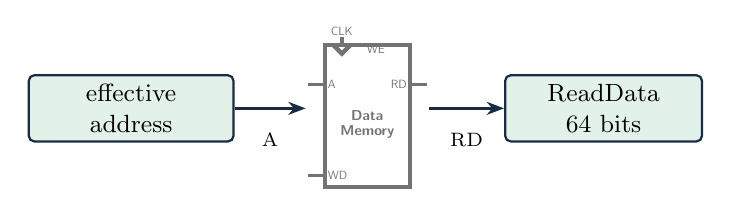
\begin{tikzpicture}[font=\small]
  \node[logic,minimum width=2.6cm] (addr) at (0,0) {effective\\address};
  \node[draw=none,inner sep=0pt] (mem) at (3.0,0) {\DataMemSymbol[0.36]};
  \node[logic,minimum width=2.5cm] (data) at (6.0,0) {ReadData\\64 bits};
  \draw[bus] (addr)--node[below=5pt,font=\scriptsize]{A}(mem);
  \draw[bus] (mem)--node[below=5pt,font=\scriptsize]{RD}(data);
\end{tikzpicture}
\end{center}
\vspace{0.2cm}
The memory read value becomes the candidate writeback value for \code{x7}.
\end{frame}

% ============================================================
% Slide 26
% ============================================================

\begin{frame}{Step 7: Write Back and Update PC}
\begin{center}
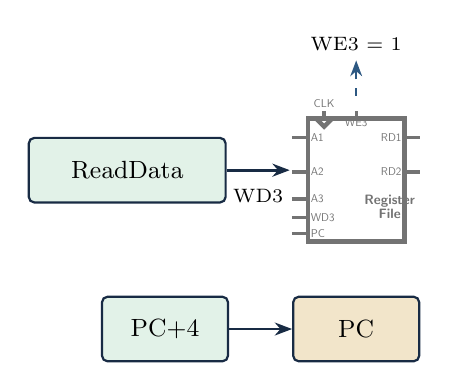
\begin{tikzpicture}[node distance=0.8cm,font=\small]
  \node[logic,minimum width=2.5cm] (data) {ReadData};
  \node[draw=none,inner sep=0pt,right=of data] (rf) {\RegFileSymbol[0.34]};
  \node[state,below=0.65cm of rf,minimum width=1.6cm] (pc) {PC};
  \node[logic,left=of pc,minimum width=1.6cm] (pc4) {PC+4};
  \draw[bus] (data)--node[below=3pt,font=\scriptsize]{WD3}(rf.west);
  \draw[ctrl] (rf.north)--++(0,0.45) node[above,font=\scriptsize]{WE3 = 1};
  \draw[arr] (pc4)--(pc);
\end{tikzpicture}
\end{center}
\vspace{0.2cm}
At the clock edge, \code{x7} receives the loaded value and the PC receives \(PC+4\).
\end{frame}

% ============================================================
% Slide 27
% ============================================================

\begin{frame}{Load Path Control Settings}
\small
\begin{center}
\rowcolors{2}{blue!6}{white}
\begin{tabular}{lll}
\toprule
Signal & Setting for \code{ldr x7, [x5, \#8]} & Effect \\
\midrule
\code{RegWrite} & 1 & write loaded value to \code{x7} \\
\code{MemWrite} & 0 & do not write data memory \\
\code{MemToReg} & 1 & writeback comes from data memory \\
\code{ALUSrc} & 1 & ALU second input is the extended offset \\
\code{ALUControl} & add & compute base + offset \\
\code{ImmSrc} & load/store scaled & produce byte offset 8 \\
\code{PCSrc} & 0 & next PC is \(PC+4\) \\
\bottomrule
\end{tabular}
\end{center}
\vspace{0.1cm}
These control values select one path through the same hardware.
\end{frame}

% ============================================================
% Slide 28
% ============================================================

\sectiondivider{PART 4}{Extending the Datapath}

% ============================================================
% Slide 29
% ============================================================

\begin{frame}{Store Path: \texttt{str x7, [x5, \#8]}}
\small
\code{str x7, [x5, \#8]} uses the same address calculation as the load.

\vspace{0.18cm}
\begin{center}
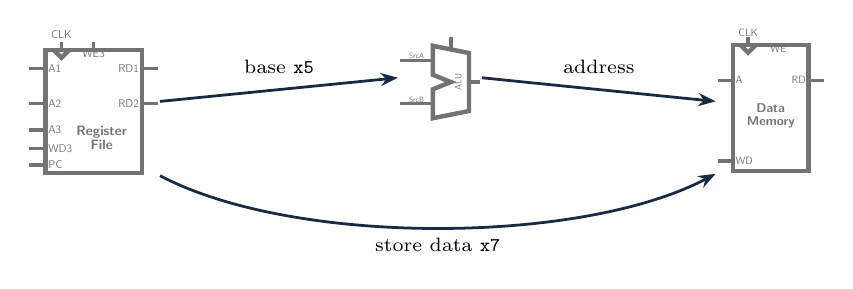
\begin{tikzpicture}[font=\small]
  \node[draw=none,inner sep=0pt] (rf) at (0,0) {\RegFileSymbol[0.34]};
  \node[draw=none,inner sep=0pt] (alu) at (4.4,0.3) {\ALUSymbol[0.23]};
  \node[draw=none,inner sep=0pt] (mem) at (8.6,0) {\DataMemSymbol[0.32]};
  \draw[bus] (rf.east)--node[above=2pt,font=\scriptsize]{base \code{x5}}(alu.west);
  \draw[bus] (alu.east)--node[above=2pt,font=\scriptsize]{address}(mem.west);
  \draw[bus] (rf.south east).. controls +(1.7,-0.9) and +(-1.7,-0.9) .. node[below,font=\scriptsize]{store data \code{x7}}(mem.south west);
\end{tikzpicture}
\end{center}
\vspace{0.12cm}
\begin{itemize}\setlength{\itemsep}{5pt}
  \item \code{Rt = x7} is read from the register file as store data.
  \item \code{MemWrite = 1} and \code{RegWrite = 0}.
\end{itemize}
\end{frame}

% ============================================================
% Slide 30
% ============================================================

\begin{frame}{Register ALU Path: \texttt{add x1, x2, x3}}
\begin{center}
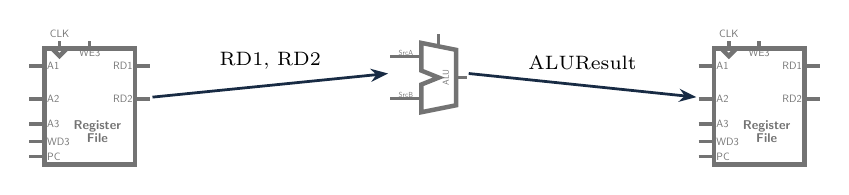
\begin{tikzpicture}[font=\small]
  \node[draw=none,inner sep=0pt] (rf) at (0,0) {\RegFileSymbol[0.32]};
  \node[draw=none,inner sep=0pt] (alu) at (4.3,0.3) {\ALUSymbol[0.22]};
  \node[draw=none,inner sep=0pt] (wb) at (8.5,0) {\RegFileSymbol[0.32]};
  \draw[bus] (rf.east)--node[above=2pt,font=\scriptsize]{RD1, RD2}(alu.west);
  \draw[bus] (alu.east)--node[above=2pt,font=\scriptsize]{ALUResult}(wb.west);
\end{tikzpicture}
\end{center}
\vspace{0.2cm}
\begin{itemize}\setlength{\itemsep}{6pt}
  \item No data memory access is needed.
  \item \code{MemToReg = 0}, so the writeback value comes from the ALU.
  \item \code{ALUSrc = 0}, so the ALU second operand comes from the register file.
\end{itemize}
\end{frame}

% ============================================================
% Slide 31
% ============================================================

\begin{frame}{Immediate ALU Path: \texttt{add x1, x2, \#3}}
\begin{center}
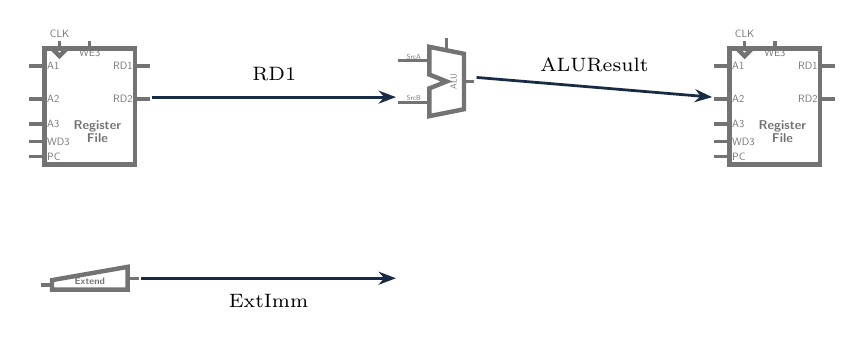
\begin{tikzpicture}[font=\small]
  \node[draw=none,inner sep=0pt] (rf) at (0,1.1) {\RegFileSymbol[0.32]};
  \node[draw=none,inner sep=0pt] (imm) at (0,-1.2) {\ExtendSymbol[0.24]};
  \node[draw=none,inner sep=0pt] (alu) at (4.4,1.35) {\ALUSymbol[0.22]};
  \node[draw=none,inner sep=0pt] (wb) at (8.7,1.1) {\RegFileSymbol[0.32]};
  \draw[bus] (rf.east)--node[above=2pt,font=\scriptsize]{RD1}(alu.west |- rf.east);
  \draw[bus] (imm.east)--node[below=2pt,font=\scriptsize]{ExtImm}(alu.west |- imm.east);
  \draw[bus] (alu.east)--node[above=2pt,font=\scriptsize]{ALUResult}(wb.west);
\end{tikzpicture}
\end{center}
\vspace{0.15cm}
For immediate ALU instructions, \code{ALUSrc = 1} selects the immediate generator output.
\end{frame}

% ============================================================
% Slide 32
% ============================================================

\begin{frame}{Second Register Source Selection}
\small
AArch64 register fields are not all used the same way across instruction families.

\vspace{0.16cm}
\begin{center}
\rowcolors{2}{blue!6}{white}
\begin{tabular}{lll}
\toprule
Instruction form & Register file read port 1 & Register file read port 2 \\
\midrule
\code{add xD, xN, xM} & \code{Rn} bits 9:5 & \code{Rm} bits 20:16 \\
\code{add xD, xN, \#imm} & \code{Rn} bits 9:5 & not used \\
\code{ldr xT, [xN, \#imm]} & \code{Rn} bits 9:5 & not used \\
\code{str xT, [xN, \#imm]} & \code{Rn} bits 9:5 & \code{Rt} bits 4:0 \\
\bottomrule
\end{tabular}
\end{center}
\vspace{0.12cm}
A small multiplexer selects whether the second read address comes from \code{Rm} or \code{Rt}.
\end{frame}

% ============================================================
% Slide 33
% ============================================================

\begin{frame}{Branch Path: \texttt{b label}}
\begin{center}
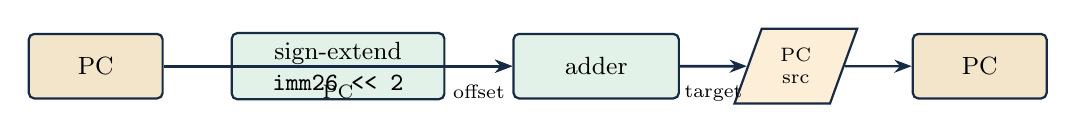
\begin{tikzpicture}[node distance=0.85cm,font=\small]
  \node[state,minimum width=1.7cm] (pc) {PC};
  \node[logic,right=of pc,minimum width=2.7cm] (imm) {sign-extend\\\code{imm26 << 2}};
  \node[logic,right=of imm,minimum width=2.1cm] (add) {adder};
  \node[mux,right=of add] (mux) {PC\\src};
  \node[state,right=of mux,minimum width=1.7cm] (newpc) {PC};
  \draw[bus] (pc)--node[below=3pt,font=\scriptsize]{PC}(add);
  \draw[bus] (imm)--node[below=3pt,font=\scriptsize]{offset}(add);
  \draw[bus] (add)--node[below=3pt,font=\scriptsize]{target}(mux);
  \draw[arr] (mux)--(newpc);
\end{tikzpicture}
\end{center}
\vspace{0.2cm}
A branch replaces \(PC+4\) with a PC-relative target address.
\end{frame}

% ============================================================
% Slide 34
% ============================================================

\sectiondivider{PART 5}{Control Signals and Timing}

% ============================================================
% Slide 35
% ============================================================

\begin{frame}{Control Signals}
\small
\begin{center}
\rowcolors{2}{blue!6}{white}
\begin{tabular}{ll}
\toprule
Signal & Meaning \\
\midrule
\code{RegWrite} & enable a write to the register file \\
\code{MemWrite} & enable a write to data memory \\
\code{MemToReg} & choose memory data or ALU result for writeback \\
\code{ALUSrc} & choose register data or immediate as ALU input B \\
\code{ALUControl} & select add, subtract, and, or other ALU operation \\
\code{ImmSrc} & select the immediate-extension mode \\
\code{Read2Src} & choose \code{Rm} or \code{Rt} for the second register read \\
\code{PCSrc} & choose sequential PC or branch target \\
\bottomrule
\end{tabular}
\end{center}
\end{frame}

% ============================================================
% Slide 36
% ============================================================

\begin{frame}{Example Control Settings}
\scriptsize
\begin{center}
\rowcolors{2}{blue!6}{white}
\begin{adjustbox}{max width=\textwidth}
\begin{tabular}{lllllllll}
\toprule
Instruction & RegW & MemW & MemToReg & ALUSrc & ALU & ImmSrc & Read2Src & PCSrc \\
\midrule
\code{ldr xT, [xN, \#imm]} & 1 & 0 & 1 & 1 & add & load/store & -- & 0 \\
\code{str xT, [xN, \#imm]} & 0 & 1 & X & 1 & add & load/store & \code{Rt} & 0 \\
\code{add xD, xN, xM} & 1 & 0 & 0 & 0 & add & -- & \code{Rm} & 0 \\
\code{sub xD, xN, xM} & 1 & 0 & 0 & 0 & sub & -- & \code{Rm} & 0 \\
\code{add xD, xN, \#imm} & 1 & 0 & 0 & 1 & add & add/sub imm & -- & 0 \\
\code{b label} & 0 & 0 & X & X & add & branch & -- & 1 \\
\bottomrule
\end{tabular}
\end{adjustbox}
\end{center}
\vspace{0.12cm}
\normalsize
The entries marked \code{X} are not used by that instruction.
\end{frame}

% ============================================================
% Slide 37
% ============================================================

\begin{frame}{Single-Cycle Limitations}
\large
\begin{itemize}\setlength{\itemsep}{7pt}
  \item Hardware is easy to reason about, but timing is inefficient.
  \item Every instruction waits for the worst-case datapath delay.
  \item Simple instructions cannot finish early.
  \item Some hardware must be duplicated when two values are needed in the same cycle.
  \item The next topic reuses the same datapath ideas but overlaps instructions in a pipeline.
\end{itemize}
\end{frame}

% ============================================================
% Slide 38
% ============================================================

\sectiondivider{PART 6}{Summary and Review}

% ============================================================
% Slide 39
% ============================================================

\begin{frame}{Topic 8: Summary}
\large
\begin{itemize}\setlength{\itemsep}{7pt}
  \item A single-cycle datapath computes the next architectural state in one clock period.
  \item State elements store the PC, registers, memory contents, and flags.
  \item The \code{ldr x7, [x5, \#8]} path uses instruction fetch, register read, immediate scaling, ALU address calculation, memory read, and register writeback.
  \item The same datapath is extended with multiplexers and control signals for stores, ALU instructions, and branches.
\end{itemize}
\end{frame}

% ============================================================
% Slide 40
% ============================================================

\begin{frame}{Self-Test Questions: Datapath Basics}
\begin{enumerate}\setlength{\itemsep}{7pt}
  \item In a single-cycle datapath, when are state elements updated?
  \item Why is the PC modeled separately from the AArch64 general-purpose register file?
  \item For \code{ldr x7, [x5, \#8]}, which register supplies the base address?
  \item Why is the encoded \code{imm12} equal to 1 rather than 8 for that instruction?
  \item What is the role of the ALU in a load or store instruction?
\end{enumerate}
\end{frame}

% ============================================================
% Slide 41
% ============================================================

\begin{frame}{Self-Test Questions: Control and Timing}
\begin{enumerate}\setlength{\itemsep}{7pt}
  \item Which control signal distinguishes a register ALU operand from an immediate ALU operand?
  \item Why does \code{str} assert \code{MemWrite} but not \code{RegWrite}?
  \item What value does \code{MemToReg} select for a load?
  \item Why does a single-cycle implementation have a long clock period?
  \item Which datapath components are used by \code{add x1, x2, x3} but not by \code{b label}?
\end{enumerate}
\end{frame}

% ============================================================
% Slide 42
% ============================================================

\begin{frame}{Looking Ahead}
\large
\begin{itemize}\setlength{\itemsep}{8pt}
  \item The single-cycle datapath shows the full instruction path in one cycle.
  \item Pipelining splits that path into stages so several instructions can be in progress at once.
  \item The next topic uses the same fetch, decode, execute, memory, and writeback structure to build the 5-stage RISC pipeline.
  \item Hazards appear when overlapped instructions need the same data or control decision.
\end{itemize}
\end{frame}

\end{document}